\documentclass{beamer}
\usepackage[utf8]{inputenc}
\usepackage{listings}
\usepackage{listingsutf8}
\usepackage{hyperref}
\usepackage{wrapfig}
\usepackage[absolute,overlay]{textpos}

\usetheme{Berkeley}

\title{NodeMCU}
\author{Fabiano Sardenberg Kuss}
\date{\today}


\lstset{
    language=c++,
    extendedchars=false,
    backgroundcolor=\color{gray!30},
    framextopmargin=2pt,
    framexbottommargin=2pt,
    rulecolor=\color{black!30},
    inputencoding=utf8
}


\begin{document}

\section{Introdução}

\begin{frame}[fragile, t]
\frametitle{Introdução}

A plataforma NodeMCU é uma placa open source baseada nas funcionalidade providas pelo chip de 
baixo custo com suporte a redes sem fio 802.11 ESP8266 que utiliza o microprocessador Xtensa.

Esta plataforma oferece um ambiente adequado para o desenvolvimento de dispositivos que 
implementam funcionalidades para atuarem em um conceito de IoT de forma simples. Pode
ser visto como uma evolução da estratégia de desenvolvimento utilizando Arduino

\begin{picture}(0,0)
    \put(20, -75){
    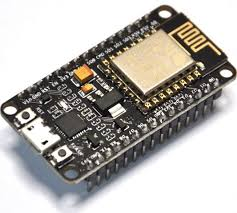
\includegraphics[scale=0.4]{imgs/nodeMCU.png}
    }
    \put(150, -60){
    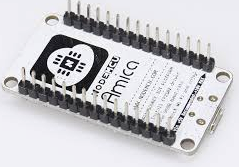
\includegraphics[scale=0.4]{imgs/back_node_mcu.png}
    }
\end{picture}

\end{frame}

\begin{frame}[fragile, t]
\frametitle{Introdução}

A plataforma NodeMCU é um kit de desenvolvimento open source baseada nas funcionalidade providas pelo chip de 
baixo custo com suporte a redes sem fio 802.11 ESP8266 que utiliza o microprocessador Xtensa.

Esta plataforma oferece um ambiente adequado para o desenvolvimento de dispositivos que 
implementam funcionalidades para atuarem em um conceito de IoT de forma simples. Pode
ser visto como uma evolução da estratégia de desenvolvimento utilizando Arduino

\begin{picture}(0,0)
    \put(20, -75){
    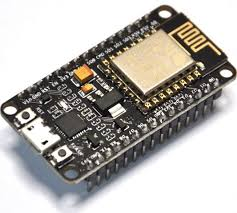
\includegraphics[scale=0.4]{imgs/nodeMCU.png}
    }
    \put(150, -60){
    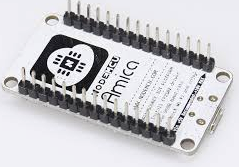
\includegraphics[scale=0.4]{imgs/back_node_mcu.png}
    }
\end{picture}

\end{frame}


\begin{frame}[fragile, t]
\frametitle{Apresentando a Placa}


\begin{picture}(0,225)
    \put(20, 15){
    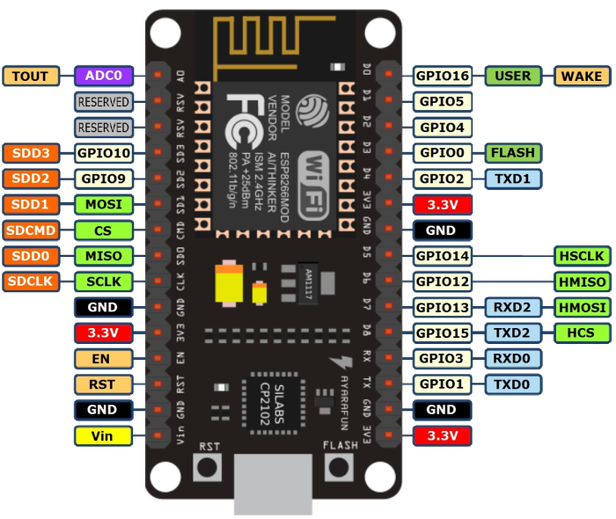
\includegraphics[scale=0.4]{imgs/pinout.png}
    }
\end{picture}

\end{frame}

\begin{frame}[fragile, t]
\frametitle{ESP8266}

\begin{picture}(0,0)
    \put(120, -200){
    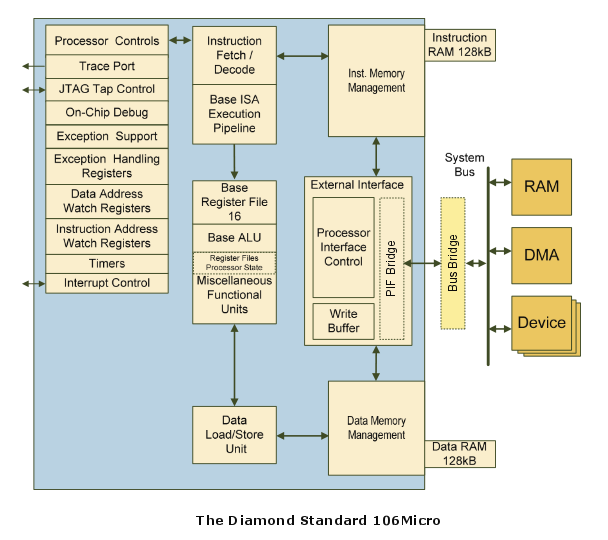
\includegraphics[scale=0.3]{imgs/xtensa-l106.png}
    }
\end{picture}


\begin{itemize}
\item Microcontrolador: Xtensa L106 (32-bit) 80Mhz
\item Memória Interna: 128K para instruções; 128K para dados
\item Memória Flash: 4Mb.
\item I/O: 16 Pinos GPIO
\item Tensão: 3.3 VDC
\item WI-FI: 802.11 b/g/n
\end{itemize}

\end{frame}




\section{Usando o Arduino IDE}
\subsection{Baixando e Instalando o Arduino IDE}

\begin{frame}[fragile]
\frametitle{Instalando o Arduino IDE}


Download da IDE em https://www.arduino.cc/en/Main/Software

Extrair o arquivo com

\begin{lstlisting}
tar xvf arduino-1.8.X-linux64.tar.xz
\end{lstlisting}

Ir para a pasta e iniciar a IDE
\begin{lstlisting}
cd arduino-1.8.X 
./arduino
\end{lstlisting}


Para adicionar suporte a placa ESP12 e NodeMCU é necessário carregar o compilador e configurações para 
compilação, geração da flash e copiar o arquivo gerado para o processador. 

\end{frame}



\begin{frame}[fragile]
\frametitle{Instalando o Arduino IDE}

\begin{picture}(0,0)
    \put(0, -20){
    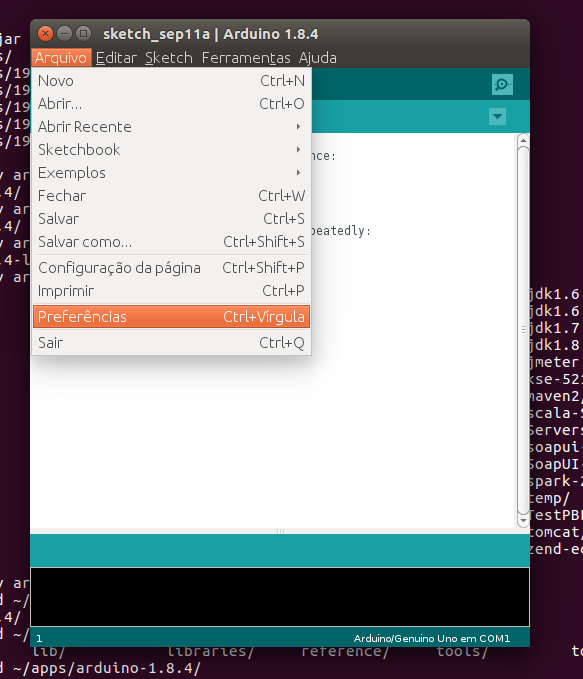
\includegraphics[scale=0.17]{imgs/arquivo_preferencias.png}
    }
    \put(120, -100){
    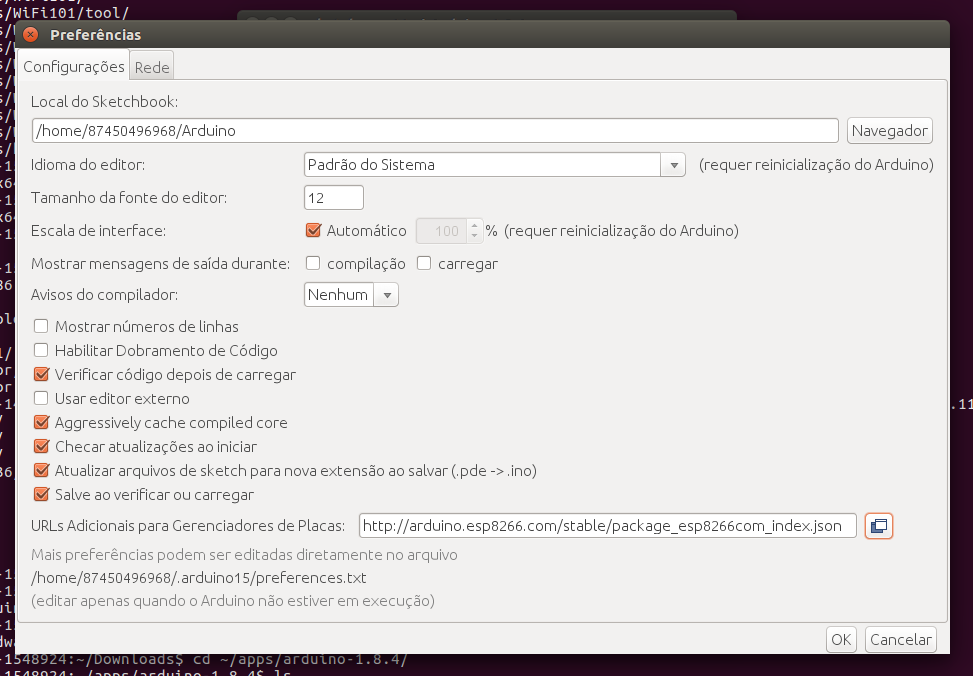
\includegraphics[scale=0.17]{imgs/preferencias.png}
    }
\end{picture}

\begin{textblock*}{50mm}(60mm,0.27\textheight)
    Selecionar o submenu Preferências pelo menu Arquivo, será aberta uma janela com várias opções de configuração
\end{textblock*}


\begin{textblock*}{40mm}(17mm,0.80\textheight)
    No campo URLs Adicionais para Gerenciador de Placas deve ser inserido o seguinte valor
    http://arduino.esp8266.com/stable/package\_esp8266com\_index.json
\end{textblock*}


\end{frame}

\subsection{Configurando o Arduino IDE}

\begin{frame}[fragile]
\frametitle{Configurando suporte para ESP12 e NodeMCU}

\begin{picture}(0,0)
    \put(0, -20){
    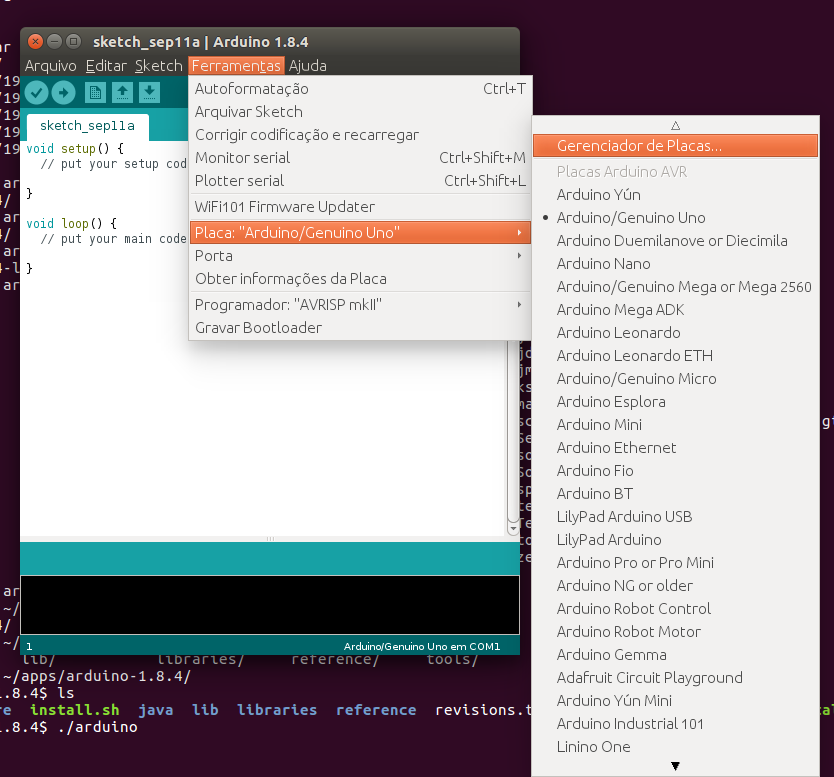
\includegraphics[scale=0.15]{imgs/gerenciador.png}
    }
    \put(150, -90){
    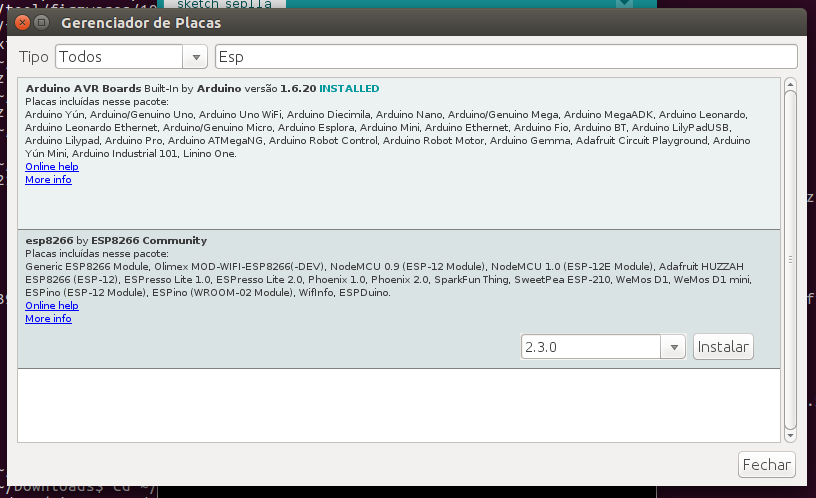
\includegraphics[scale=0.18]{imgs/import_esp.png}
    }
\end{picture}

\begin{textblock*}{50mm}(75mm,0.25\textheight)
    Selecionar o submenu Gerenciador de Placas a partir pelo menu Ferramentas, submenu Placa
\end{textblock*}


\begin{textblock*}{53mm}(20mm,0.78\textheight)
    Para facilitar a busca é possível aplicar filtros no capo Refine sua busca. O valor Esp é suficiente
    para retornar poucos resultados. Basta selecionar ESP8266 by ESP8266 Communit e instalar
\end{textblock*}


\end{frame}

\begin{frame}[fragile]
\frametitle{Configurações Finais}

\begin{picture}(0,200)
    \put(0, 30){
    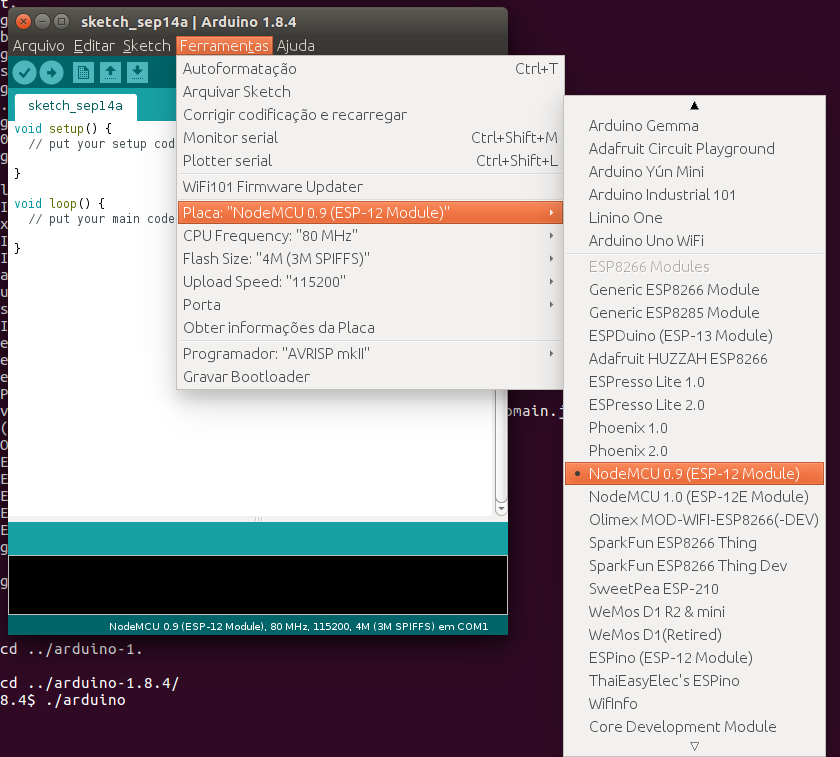
\includegraphics[scale=0.18]{imgs/board_config.png}
    }
\end{picture}

\begin{textblock*}{45mm}(80mm,0.3\textheight)
Após a seleção da placa NoceMCU 0.9 retorne ao menu ferramentas e selecione a porta USB correta
No Linux as portas de comunicação serial com o Módulo é mapeada como /dev/ttyUSBX, onde
X é um número inteiro com valor inicial 0.

Você pode verificar as portas ativas utilizando o comando ls /dev/tty*
\end{textblock*}


\end{frame}


\section{Programando com a IDE Arduino}

\begin{frame}[fragile]
\frametitle{Compilação e cópia}
\small
\begin{block}{}
Para a compilação a IDE utiliza uma coleção de programas para execução do GCC, gerando código para o 
microprocessador Xensa. Quando é feita a instalação de suporte para NodeMCU este conjunto de programas
é baixado localmente.
\end{block}

\begin{block}{}
A cópia do código binário gerado para a placa tem que ser feita passando um conjunto de instruções 
concebidas específicamente para o processador. No caso da ESP12 o programa é na realidade um firmware.
\end{block}

\begin{block}{}
Para apresentar detalhadamente o processo de compilação e cópia do programa é necessário configurar a 
IDE habilitando os campos compilação e carregar em Mostrar Mensagens de Saída na tela de prferências
(Arquivo, Preferências)
\end{block}

\end{frame}


\subsection{Estrutura da linguagem}
\begin{frame}[fragile]
\frametitle{}

A programação é feita utilizando a sintaxe da linguagem C++, podendo ser utilizadas as funções
e tipos primitivos da mesma. No entanto muitas das boas práticas utilizadas para programação
em computadores tradicionais devem ser revistas para desenvolvimento de sistemas embarcados.

\begin{itemize}
\item Duas funções que tem que existir em qualquer programa;
\begin{itemize}
\item setup()
\item loop()
\end{itemize}
\item setup() é executado na inicialização do programa, é equivamente a main()
\item loop(), é chamado após a conclusão da função setup() é é um loop infinito
\end{itemize}

\end{frame}



\begin{frame}[fragile]
\frametitle{Algumas funções e constantes}

Constantes
\begin{itemize}
\item OUTPUT, INPUT
\item LOW, HIGHT
\end{itemize}

Programação para Portas
\begin{itemize}
\item pinMode(PIN, [INPUT|OUTPUT])
\item digitalWrite(PIN, [LOW|HIGH])
\item digitalRead(PIN)
\item delay(TIME\_Ms)
\end{itemize}

Comunicação Serial
\begin{itemize}
\item Serial.begin(SPEED)
\item Serial.println(DATA)
\item Serial.print(DATA)
\item Serial.available()
\item Serial.read()
\end{itemize}
\end{frame}





\begin{frame}[fragile]
\frametitle{Blick um Hello Word em IoT}

\scriptsize
\begin{lstlisting}
/*
 ESP8266 Blink by Simon Peter
 Blink the blue LED on the ESP-01 module
 This example code is in the public domain
 
*/

void setup() {
  pinMode(LED_BUILTIN, OUTPUT);     
}

void loop() {
  digitalWrite(LED_BUILTIN, LOW);   
  delay(1000);
  digitalWrite(LED_BUILTIN, HIGH);
  delay(2000);
}

\end{lstlisting}

\end{frame}


\begin{frame}[fragile]
\frametitle{Blick com 2 Leds}

\scriptsize
\begin{lstlisting}

int EXTLED = 5; //Aqui devemos usar o GPIO
int count = 0;

void setup() {
  pinMode(LED_BUILTIN, OUTPUT);     
  pinMode(EXTLED, OUTPUT);     
}

void loop() {
       
  if(count %2 == 0){
    digitalWrite(EXTLED, HIGH);
    digitalWrite(LED_BUILTIN, LOW);
  }else{
    digitalWrite(EXTLED, LOW);
    digitalWrite(LED_BUILTIN, HIGH);
  }
  count++;
  delay(1000);
}

\end{lstlisting}

\end{frame}

\subsection{Monitor Serial}

\begin{frame}[fragile]
\frametitle{Monitor Serial}

\begin{picture}(0,250)
    \put(0, 110){
    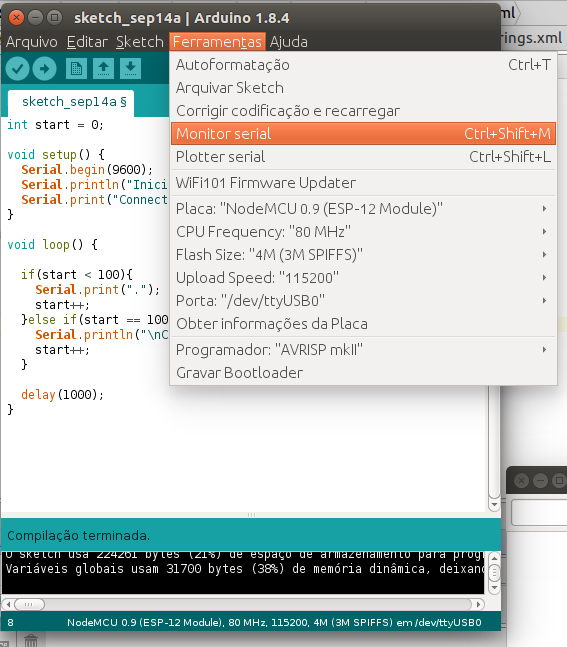
\includegraphics[scale=0.18]{imgs/open_monitor_serial.png}
    }
    \put(40, 30){
    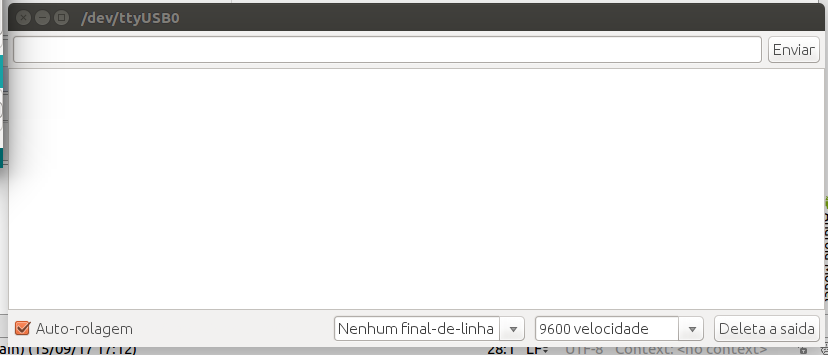
\includegraphics[scale=0.25]{imgs/monitor_serial.png}
    }
\end{picture}

\begin{textblock*}{45mm}(70mm,0.3\textheight)
A IDE Arduino oferece uma interface que permite ler e enviar dados para a saída serial. Quando está
é habilitada passa a comunicar-se com a interface na porta selecionada.
\end{textblock*}


\end{frame}




\begin{frame}[fragile]
\frametitle{Comunicação serial}

\scriptsize
\begin{lstlisting}

int start = 0;

void setup() {
  Serial.begin(9600); 
  Serial.println("Iniciando");
  Serial.print("Connectando com");
}

void loop() {

  if(start < 100){
    Serial.print(".");
    start++;
  }else if(start == 100){
    Serial.println("\nConnected");
    start++;
  }

  delay(1000);
}

\end{lstlisting}

\end{frame}


\begin{frame}[fragile]
\frametitle{Comunicação serial}

\tiny
\begin{lstlisting}
String data;
int porta = 0;

void setup() {
  Serial.begin(9600);
  delay(500);
  Serial.write("Digite algo:\n");
  
}

void loop() {
  if (Serial.available() > 0) {
    
    data = Serial.readString(); 
    Serial.print("Digitado: ");
    Serial.println(data);

    Serial.println("Digite um número: ");
    while(Serial.available() <= 0){}
    porta = Serial.readString().toInt();
    Serial.print(porta, HEX); 
    Serial.write("\nDigite algo:\n");
  }
  delay(10);
}
\end{lstlisting}

\end{frame}




\subsection{Utilizando exemplos}
\begin{frame}[fragile]
\frametitle{}

\begin{picture}(0,150)
    \put(30, 30){
    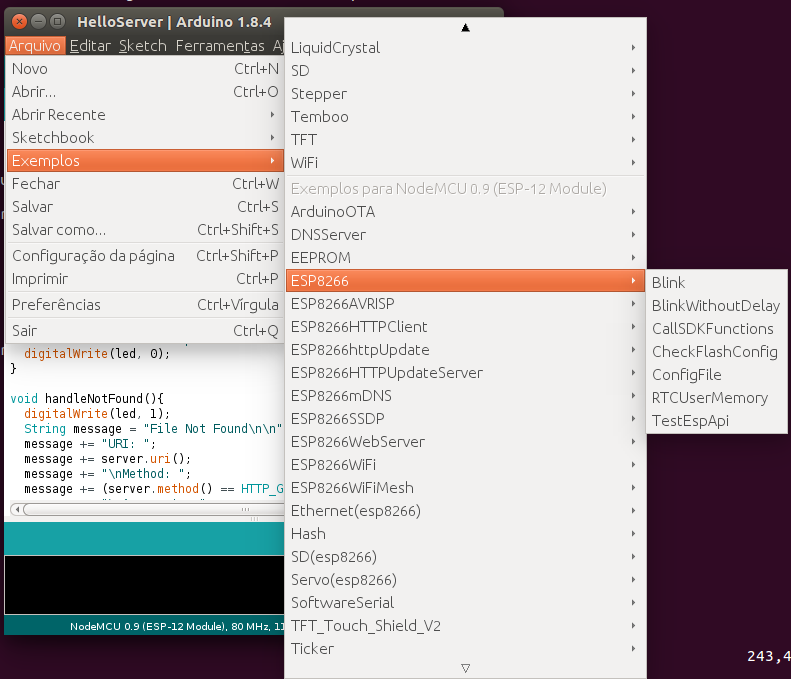
\includegraphics[scale=0.20]{imgs/examples.png}
    }
\end{picture}

\begin{textblock*}{100mm}(20mm,0.9\textheight)
Quando é baixado o suporte para ESP na IDE Arduino são configurados vários exemplos de programas que 
ajudam não apenas iniciantes mas podem ser uma boa ferramenta para funcionalidades necessárias durante
o desenvolvimento de aplicações.

\end{textblock*}

\end{frame}

\subsection{Incluindo bibliotecas}
\begin{frame}[fragile]
\frametitle{}

\begin{block}{}
Para facilitar a implementação de alguns módulos é possível utilizar bibliotecas especialmente desenvolvidas
para estes produtos. Estes programas podem ser obtidor utilizando o Sketch acessando o menu Sketch,
Incluir Biblioteca, Gerenciar Biblioteca.
\end{block}


\begin{block}{}
Alternativamente é possível baixar os arquivos do módulo que deseja instalar e extrair o mesmo na pasta 
libraries no diretório de instalação da IDE.
\end{block}

\end{frame}


\section{Funcionalidades WI-FI}

\begin{frame}[fragile]
\frametitle{WI-FI}

Classes
\begin{itemize}
\item pinMode(PIN, [INPUT|OUTPUT])
\item digitalWrite(PIN, [LOW|HIGH])
\item digitalRead(PIN)
\item delay(TIME\_Ms)
\end{itemize}

WI-FI (definidos em ESP8266WiFi.h)
\begin{itemize}
\item WiFi.begin(SSID, SENHA);
\item WiFi.status()
\item WiFi.localIP()
\end{itemize}

\end{frame}

\begin{frame}[fragile]
\frametitle{Conectar ao AP}

\tiny
\begin{lstlisting}
#include <ESP8266WiFi.h>

const char* ssid     = "ssid";
const char* password = "senha_do_ssid";

void setup() {
  Serial.begin(9600);
  delay(10);
  Serial.print("Conectando com: ");
  Serial.println(ssid);
 
  WiFi.begin(ssid, password);

  while (WiFi.status() != WL_CONNECTED) {
    delay(500);
    Serial.print(".");
  }

  Serial.println("");
  Serial.println("WiFi conectado");  
  Serial.println("IP address: ");
  Serial.println(WiFi.localIP());
}


void loop() {

}
\end{lstlisting}

\end{frame}


\begin{frame}[fragile]
\frametitle{Configurar como AP}

\tiny
\begin{lstlisting}
#include <ESP8266WiFi.h>

const char* ssid     = "MeuAP";
const char* password = "minhasenha";
IPAddress IP(192,168,200,1);
IPAddress net(255,255,255,0);

void setup() {
  Serial.begin(9600);
  delay(10);
  Serial.print("Iniciando serviço: ");
  
  WiFi.mode(WIFI_AP); 
  WiFi.softAPConfig(IP, IP, net)
  WiFi.softAP(ssid, password);

  while (WiFi.status() != WL_CONNECTED) {
    delay(500);
    Serial.print(".");
  }

  Serial.println("IP address: ");
  Serial.println(WiFi.localIP());
}


void loop() {
    Serial.println(WiFi.localIP());
}
\end{lstlisting}

\end{frame}

\begin{frame}[fragile]
\frametitle{Atendendo requisições (setup)}

\tiny
\begin{lstlisting}
#include <ESP8266WiFi.h>

const char* ssid     = "MeuAP";
const char* password = "minhasenha";
IPAddress IP(192,168,200,1);
IPAddress net(255,255,255,0);
int EXTLED = 5;

WiFiServer server(80);

void setup() {
  Serial.begin(9600);
  delay(10);

  WiFi.mode(WIFI_AP); 
  WiFi.softAPConfig(IP, IP, net);
  WiFi.softAP(ssid, password);
  delay(1000);
  server.begin();

  pinMode(LED_BUILTIN, OUTPUT);
  pinMode(EXTLED, OUTPUT);

}


\end{lstlisting}

\end{frame}


\begin{frame}[fragile]
\frametitle{Atendendo requisições (loop)}

\tiny
\begin{lstlisting}

void loop() {
    WiFiClient client = server.available();
    if(!client)
        return;
        
    while(!client.available())
        delay(1);
    Serial.println("Conexão recebida");
    client.println("HTTP/1.1 200 OK");
    client.println("Content-Type: text/html");
    client.println("");//Fim do cabecalho http \n\r
    client.println("<html><meta charset='utf-8'/><h1>Olá cliente</h1></html>");

    digitalWrite(EXTLED, HIGH);
    digitalWrite(LED_BUILTIN, HIGH);
    delay(1000);
    digitalWrite(EXTLED, LOW);
    digitalWrite(LED_BUILTIN, LOW);

    delay(10);
  
}
 
\end{lstlisting}
\end{frame}


\begin{frame}[fragile]
\frametitle{Atendendo requisições (loop)}

\tiny
\begin{lstlisting}

void loop() {
    WiFiClient client = server.available();
    if(!client)
        return;

    while(!client.available()){

      if (Serial.available() > 0) {
        data = Serial.readString();
        Serial.print("Digitado: ");
        Serial.println(data);  
        continue;
      }
    }

    response = "<html><meta charset='utf-8'/><h1>Olá cliente "+data+"</h1></html>";
    Serial.println("Conexão recebida");
    client.println("HTTP/1.1 200 OK");
    client.println("Content-Type: text/html");
    client.println("");//Fim do cabecalho http \n\r
    client.println(response);


    delay(10);  
}
 
\end{lstlisting}
\end{frame}

\begin{frame}[fragile]
\frametitle{Passando parâmetros (loop)}

\tiny
\begin{lstlisting}
void loop() {
    WiFiClient client = server.available();
    if(!client)
        return;
        
    while(!client.available())
        delay(1);


    String request = client.readStringUntil('\r');
    String response = "<html><style>input{width:500px;height:180px;margin-bottom:40px}}</style>";
    response += "<input type='button' value ='On' onclick='location.href=\"?l=on\"'/><br>";
    response += "<input type='button' value ='Off' onclick='location.href=\"?l=off\"'/>";
    client.flush();

    Serial.println(request);

    if(request.indexOf("?l=on") >= 0){
        digitalWrite(EXTLED, HIGH);
    }else if(request.indexOf("?l=off") >= 0){
        digitalWrite(EXTLED, LOW);
    }

    Serial.println("Conexão recebida");
    client.println("HTTP/1.1 200 OK");
    client.println("Content-Type: text/html");
    client.println("");//Fim do cabecalho http \n\r
    client.println(response);


    delay(10);
 
}
\end{lstlisting}
\end{frame}



\begin{frame}[fragile]
\frametitle{Melhorando a interface (loop)}

\tiny
\begin{lstlisting}

void loop() {
    WiFiClient client = server.available();
    if(!client)
        return;
        
    while(!client.available())
        delay(1);


    String request = client.readStringUntil("\n");
    String response = "<html><meta charset='utf-8'/><h1>Nada a fazer</h1></html>";
    client.flush();

    if(request.indexOf("?l=on") > 0){
        digitalWrite(EXTLED, HIGH);
        response = "<html><meta charset='utf-8'/><h1>Luz Acesa</h1></html>";
    }else if(request.indexOf("?l=off") > 0)
        response = "<html><meta charset='utf-8'/><h1>Luz Acesa</h1></html>";
    }
        
    Serial.println("Conexão recebida");
    client.println("HTTP/1.1 200 OK");
    client.println("Content-Type: text/html");
    client.println("");//Fim do cabecalho http \n\r
    client.println(response);


    delay(10);
  
}
 
\end{lstlisting}
\end{frame}



\end{document}

\begin{frame}[fragile]
\frametitle{Programando em Lua}

\begin{lstlisting}
Programando em lua

Download da ferramenta que permite comunicação serial usando Python
git clone https://github.com/pyserial/pyserial.git

Download da ferramenta de flash esptool.py em
git clone https://github.com/espressif/esptool

Copiar a pasta serial de pyserial-2.7

cp -r pyserial/pyserial-2.7/serial para a pasta esptool/

Compilar o próprio módulo ou fazer download de um módulo pronto de https://github.com/nodemcu/nodemcu-firmware/releases
Para a compilação será necessário 

Copiar o firmware para o dispositivo
./esptool.py -p /dev/ttyUSB0 write_flash 0x00000 ~/Downloads/nodemcu_float_0.9.6-dev_20150704.bin
\end{lstlisting}
\end{frame}

\begin{frame}[fragile]
\frametitle{Software Livre}
\begin{lstlisting}
##Escrever um oi mundo em lua

while true do
   print("Oi Mundo")
   tmr.delay(1000 * 1000)
end

##Copiar o programa para o dispositivo

./luatool.py --port /dev/ttyUSB0  --src /tmp/script.lua --dofile


Para comunicar com a porta serial para visualizar o resultado é possível utilizar um script python
lembrando que a pasta serial tem que estar no mesmo diretório que o script

import serial
ser = serial.Serial('/dev/ttyUSB0', 9600, timeout=1)
for i in range(0,10):
    print ser.readline()

##Criando uma aplicação conectada ao Access Point

wifi.setmode(wifi.STATION)
wifi.sta.config("SSID","senha")

ip, nm, gw=wifi.sta.getip()

while true do
   print("\nIP Info:\nIP Address: "..ip.." \nNetmask: "..nm.." \nGateway Addr: "..gw.."\n")
   tmr.delay(2000*1000)
end


# Atendendo requisições WEB

srv=net.createServer(net.TCP)
srv:listen(80,function(conn)
  conn:on("receive",function(conn,payload)
    print(payload)
    conn:send("<h1>OLA ALUNO DO MINICURSO</h1>")
  end)
  conn:on("sent",function(conn) conn:close() end)
end)


#WEB e LED

LED_PIN = 1

gpio.mode(LED_PIN, gpio.OUTPUT)

wifi.setmode(wifi.STATION)
wifi.sta.config("pereskuss","meloquita")

ip, nm, gw=wifi.sta.getip()

print("\nIP Info:\nIP Address: "..ip.." \nNetmask: "..nm.." \nGateway Addr: "..gw.."\n")
tmr.delay(2000*1000)

srv=net.createServer(net.TCP)
srv:listen(80,function(conn)
  conn:on("receive",function(conn,payload)
    print(payload)
    conn:send("<h1>OLA ALUNO DO MINICURSO</h1>")
    gpio.write(LED_PIN, gpio.HIGH)
    tmr.delay(2000*1000)
    gpio.write(LED_PIN, gpio.LOW)
  end)
  conn:on("sent",function(conn) conn:close() end)
end)


get={}

if string.find(valor, "GET") == 1 then
print("OK")
end

for w in string.gfind (valor, "%S+") do
    table.insert(get, w)
end

qstring = get[2]

init=string.find(qstring, "?")

substr = string.sub(qstring, init+1, string.len(qstring))


for w, k in string.gfind(qstring, '([^&=?]-)=([^&=?]+)' ) do
print(w, k)
end


LED_PIN = 1

gpio.mode(LED_PIN, gpio.OUTPUT)

wifi.setmode(wifi.STATION)
wifi.sta.config("pereskuss","meloquita")

ip, nm, gw=wifi.sta.getip()

print("\nIP Info:\nIP Address: "..ip.." \nNetmask: "..nm.." \nGateway Addr: "..gw.."\n")
tmr.delay(2000*1000)

srv=net.createServer(net.TCP)
srv:listen(80,function(conn)
  conn:on("receive",function(conn,payload)
    print("PROCESS QS")
    for w, k in string.gfind(payload, '([^&=?]-)=([^&=?]+)' ) do print(w, k) end
    conn:send("<h1>OLA ALUNO DO MINICURSO</h1>")
    
    gpio.write(LED_PIN, gpio.HIGH)
    tmr.delay(2000*1000)
    gpio.write(LED_PIN, gpio.LOW)
  end)
  conn:on("sent",function(conn) conn:close() end)
end)
\end{lstlisting}
\end{frame}
\end{document}
